%% ++++++++++++++++++++++++++++++++++++++++++++++++++++++++++++
%% Hauptdatei, Wurzel des Dokuments
%% ++++++++++++++++++++++++++++++++++++++++++++++++++++++++++++
%
%  Gerüst:
%  * Version 0.2
%  * Dipl.-Ing. Florian Evers, florian.evers@tu-ilmenau.de
%  * Fachgebiet Kommunikationsnetze, TU Ilmenau
%  * Dipl.-Ing. Christian Tolks, christian.tolks@informatik.uni-augsburg.de
%  * Lehrstuhl für Regelungstechnik, Universität Augsburg
%
%  Für Hauptseminare, Studienarbeiten, Diplomarbeiten
%
%  Autor           : Max Mustermann
%  Letzte Änderung : 31.12.2015
%

% Headerfeld, Typ des Dokumentes, einzubindende Packages.
% Hier bei Bedarf Änderungen vornehmen.
\documentclass
[   oneside,         % oneside/twoside : Einseitiger oder zweiseitiger Druck?
    12pt,            % Bezug: 12-Punkt Schriftgröße
    DIV=15,          % Randaufteilung, siehe Dokumentation "KOMA"-Script
    BCOR=17mm,       % Bindekorrektur: Innen 17mm Platz lassen. Copyshop-getestet.
    headsepline,     % Unter Kopfzeile Trennlinie (aus: headnosepline)
    footsepline,     % Über Fußzeile Trennlinie (aus: footnosepline)
    openright,       % Neue Kapitel im zweiseitigen Druck rechts beginnen lassen
    a4paper,         % Seitenformat A4
    abstracton,      % Abstract einbinden
    listof=totoc,      % Div. Verzeichnisse ins Inhaltsverzeichnis aufnehmen
    bibliography=totoc,        % Literaturverzeichnis ins Inhaltsverzeichnis aufnehmen
    titlepage,       % Titelseite aktivieren
    headinclude,     % Seiten-Head in die Satzspiegelberechnung mit einbeziehen
    footinclude=false,     % Seiten-Foot nicht in die Satzspiegelberechnung mit einbeziehen
    numbers=noenddot, % Gliederungsnummern ohne abschließenden Punkt darstellen
%    draft,					 % Vorschauversion ohne Bilder [draft|final]
]   {scrreprt}       % Dokumentenstil: "Report" aus dem KOMA-Skript-Paket

\usepackage[active]{srcltx}
% \usepackage[activate=normal]{pdfcprot} % Optischer Randausgleich -> pdflatex!
\usepackage{microtype}
\usepackage{ifthen}
\usepackage{ngerman}
\usepackage[utf8]{inputenc}
\usepackage[T1]{fontenc}
\usepackage[T1]{url}
\usepackage{ae}
\usepackage[final]{graphicx}
\usepackage[automark]{scrlayer-scrpage}
\usepackage{setspace}
%\usepackage[first,light]{draftcopy} % Für Probedruck
\usepackage[plainpages=false,pdfpagelabels,hypertexnames=false]{hyperref}
%\usepackage{amsmath} % mathematischer Zeichensatz
%\usepackage{amssymb}
%\usepackage{siunitx}	% SI Einheiten Package
%\usepackage{makeidx} % ermöglicht Stichwortverzeichnisse
\usepackage{listings}
\usepackage{listingsutf8}
\usepackage[dvipsnames]{xcolor}
\usepackage{pdfpages}
\usepackage{gensymb}
\usepackage{eurosym}
\usepackage{booktabs}
\usepackage{caption}
\usepackage{amsmath}
\usepackage{float}
\usepackage{subcaption} 


% Definitions for Code inclusion
\lstdefinestyle{customstyle}{
	aboveskip=3mm,
	belowskip=3mm,
	showstringspaces=false,
	columns=flexible,
	backgroundcolor=\color{white},
	basicstyle={\footnotesize\ttfamily},
	numberstyle={\tiny},
	numbers=left,
	keywordstyle=\bfseries\color{BurntOrange},
	commentstyle=\itshape\color{black!50},
	identifierstyle=\color{BlueViolet},
	stringstyle=\itshape\color{ForestGreen},
	breaklines=true,
	breakatwhitespace=true,
	tabsize=4,
	xleftmargin=\parindent,
	belowcaptionskip=1\baselineskip,
	frame=L,
	captionpos=b,
	keepspaces=true,
	numbers=left,
	numbersep=6pt,
	rulecolor=\color{black},
	numberstyle=\tiny\color{black!80},
	xleftmargin=\parindent,
	frame=single
}

\lstset{literate=%
    {Ö}{{\"O}}1
    {Ä}{{\"A}}1
    {Ü}{{\"U}}1
    {ß}{{\ss}}1
    {ü}{{\"u}}1
    {ä}{{\"a}}1
    {ö}{{\"o}}1
	{~}{{\textasciitilde}}1
	{°}{{\degree}}1
}

\newcommand{\includeC}[2]{\lstinputlisting[escapechar=, language=C++, style=customstyle, caption=#2]{#1} \bigskip}

\newcommand{\includeLang}[3]{\lstinputlisting[escapechar=, language=#3, style=customstyle, caption=#2]{#1} \bigskip}

% Verhindert Einrücken von Text nach Absatz
\parindent 0pt
% Update Dokument auf pdflatex v1.6, verhinder Fehlermeldung "`pdf inclusion..."'
\pdfminorversion=6
% Tiefe der Kapitelnummerierung beeinflussen
\setcounter{secnumdepth}{3} % Tiefe der Nummerierung
\setcounter{tocdepth}{3}    % Tiefe des Inhaltsverzeichnisses

% Hier in die zweite geschweifte Klammer jeweils
% die persönlichen Daten eintragen:
% \newcommand{\artderausarbeitung}{Abschlussarbeit}
% \newcommand{\namedesautors}{Max Mustermann}
% \newcommand{\titelderarbeit}{Anfertigung einer Ausarbeitung mit \LaTeX}
% \newcommand{\inventarisierungsnummer}{AA / BB / CC / DD}

% Alternativ: Eine Hauptseminararbeit hat keine Inventarisierungsnummer:
\newcommand{\artderausarbeitung}{Praktikum für Produktionstechnik}
\newcommand{\titelderarbeit}{Entwicklungsprozess eines lenkbaren Fahrzeuges\\ TEGGLA}
\newcommand{\namedesautors}{Wilfert, Paprotta, Evertz, Khodabakhsh}
\newcommand{\inventarisierungsnummer}{}

% Abkürzungsverzeichnis beeinflussen. Hier nichts ändern!
\usepackage[intoc]{nomencl}
  \let\abbrev\nomenclature
  \renewcommand{\nomname}{Abkürzungsverzeichnis und Formelzeichen}
  \setlength{\nomlabelwidth}{.25\hsize}
  \renewcommand{\nomlabel}[1]{#1 \dotfill}
  \setlength{\nomitemsep}{-\parsep}
  \makenomenclature
\usepackage[normalem]{ulem}
  \newcommand{\markup}[1]{\textbf{#1}}

% Seitenlayout festlegen. Hier nichts ändern!
\pagestyle{scrplain}
\ihead[]{\headmark}
\ohead[]{\pagemark}
\chead[]{}
\ifoot[]{\scriptsize \artderausarbeitung}
\ofoot[]{\scriptsize \namedesautors}
\cfoot[]{}
\renewcommand{\titlepagestyle}{scrheadings}
\renewcommand{\partpagestyle}{scrheadings}
\renewcommand{\chapterpagestyle}{scrheadings}
\renewcommand{\indexpagestyle}{scrheadings}

% Abschnittsweise Nummerierung anstatt fortlaufend. Hier nichts ändern!
\makeatletter
\@addtoreset{equation}{chapter}
\@addtoreset{figure}{chapter}
\@addtoreset{table}{chapter}
\renewcommand\theequation{\thechapter.\@arabic\c@equation}
\renewcommand\thefigure{\thechapter.\@arabic\c@figure}
\renewcommand\thetable{\thechapter.\@arabic\c@table}
\makeatother

% Quelltextrahmen, klein. Hier nichts ändern!
\newsavebox{\inhaltkl}
\def\rahmenkl{\sbox{\inhaltkl}\bgroup\small\renewcommand{\baselinestretch}{1}\vbox\bgroup\hsize\textwidth}
\def\endrahmenkl{\par\vskip-\lastskip\egroup\egroup\fboxsep3mm%
\framebox[\textwidth][l]{\usebox{\inhaltkl}}}

% Quelltextrahmen, normale Groesse. Hier nichts ändern!
\newsavebox{\inhalt}
\def\rahmen{\sbox{\inhalt}\bgroup\renewcommand{\baselinestretch}{1}\vbox\bgroup\hsize\textwidth}
\def\endrahmen{\par\vskip-\lastskip\egroup\egroup\fboxsep3mm%
\framebox[\textwidth][l]{\usebox{\inhalt}}}

% Trennvorschläge für falsch getrennte Wörter.
% Wird häufig bei eingedeutschen Wörtern benötigt, da LaTeX hierbei
% gerne falsch trennt. Alternativ kann auch im Fliesstext ein
% Trennvorschlag per "\-" hinterlegt werden, bspw.:
% Die Hard\-ware besteht aus A und B.
\hyphenation{
Hard-ware
}

% Sonstige Befehlsdefinitionen hier ablegen.
\newcommand{\entspricht}{\stackrel{\wedge}{=}}
\clubpenalty = 10000 \widowpenalty = 10000 \displaywidowpenalty = 10000 % Strafpunkte bei schlechten Absätzen

\begin{document}
\onehalfspacing
%% ++++++++++++++++++++++++++++++++++++++++++++++++++++++++++++
%% Titelblatt
%% ++++++++++++++++++++++++++++++++++++++++++++++++++++++++++++
%
%  Ger�st:
%  * Version 0.2
%  * Dipl.-Ing. Florian Evers, florian.evers@tu-ilmenau.de
%  * Fachgebiet Kommunikationsnetze, TU Ilmenau
%  * Dipl.-Ing. Christian Tolks, christian.tolks@informatik.uni-augsburg.de
%  * Lehrstuhl f�r Regelungstechnik, Universit�t Augsburg
%
%  F�r Hauptseminare, Studienarbeiten, Diplomarbeiten
%
%  Autor           : Max Mustermann
%  Letzte �nderung : 31.12.2015
%

\begin{titlepage}
\centering
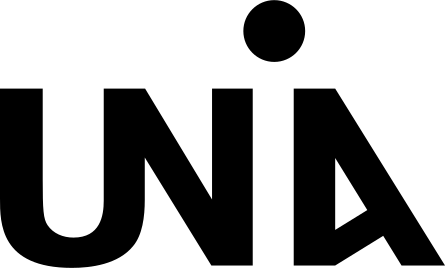
\includegraphics[scale=0.4]{bilder/Uni_Aug_Logo_Basis_pos_A}\\[3ex]
{\Large \textsc{Universit�t Augsburg}}\\[3ex]
{\Large Fakult�t f�r Angewandte Informatik}\\[3ex]
\vfill
{\Large \textbf{\artderausarbeitung}}\\[4ex]
{\large \textbf{\titelderarbeit}}\\[5ex]
\ifthenelse{\equal{\inventarisierungsnummer}{}}{}{\textbf{Inventarisierungsnummer: \inventarisierungsnummer}\\[5ex]}
\vfill
% Jonas Wilfert, Niklas Paprotta
% Johannes Evertz, Marcel Khodabakhsh
\begin{tabular}{rl}
\hline\\
vorgelegt von:          & \quad Jonas Wilfert: 1541778\\
						& \quad Niklas Paprotta\\
						& \quad Johannes Evertz: 1463672\\
						& \quad Marcel Khodabakhsh: 1333430\\[1,5ex]						
eingereicht am:         & \quad 30.\,07.\,2019\\[1,5ex]
Studiengang:            & \quad B.Sc. Ingenieurinformatik\\[1,5ex]

Anfertigung am Lehrstuhl:
                        & \quad Produktionsinformatik\\[1,5ex]
                        & \quad Fakult�t f�r Angewandte Informatik\\[1,5ex]
Verantwortlicher Professor:
                        & \quad Prof.~Dr.~Ing.~Johannes Schilp\\[1,5ex]
Wissenschaftliche Betreuer:
                        & \quad M.Sc.~Michael Aum�ller\\
                        & \quad M.Sc.~Fabian Herzer\\
						& \quad M.Sc.~Shuang Lu\\
						& \quad M.Sc.~Paul Haase\\[1,5ex]
\end{tabular}
\vfill
\end{titlepage}








% \input{vorwort.tex}
%% ++++++++++++++++++++++++++++++++++++++++++++++++++++++++++++
%% Zusammenfassung, Abstract
%% ++++++++++++++++++++++++++++++++++++++++++++++++++++++++++++
%
%  Gerüst:
%  * Version 0.10
%  * Dipl.-Ing. Florian Evers, florian.evers@tu-ilmenau.de
%  * Fachgebiet Kommunikationsnetze, TU Ilmenau
%
%  Für Hauptseminare, Studienarbeiten, Diplomarbeiten
%
%  Autor           : Max Mustermann
%  Letzte Änderung : 31.12.2004
%

\renewcommand{\abstractname}{Kurzfassung}
\begin{abstract}
Dieser Bericht soll als Dokumentation des Entwicklungsprozesses und der technischen Komponenten des TEGGLA dienen. 
Hierbei handelt es sich um ein Fahrzeugs, welches durch die besonderen Mecanum-Räder mehr Freiheitsgrade hat als ein konventionelles Automobil.
Dieses wurde im Rahmen des Praktikum für Produktionstechnik entwickelt und gebaut.
\end{abstract}


% Inhaltsverzeichnis
\cleardoublepage % Seitenumbruch erzwingen vor Änderung des Nummerierungsstils
\pagenumbering{roman} % Nummerierung der Seiten ab hier: i, ii, iii, iv...
\pagestyle{scrheadings} % Ab hier mit Kopf- und Fusszeile
\tableofcontents

% Die einzelnen Kapitel
\cleardoublepage % Seitenumbruch erzwingen vor Änderung des Nummerierungsstils
\pagenumbering{arabic} % Nummerierung der Seiten ab hier: 1, 2, 3, 4...
%% ++++++++++++++++++++++++++++++++++++++++++++++++++++++++++++
%% Kapitel 1: Einleitung, Problemstellung
%% ++++++++++++++++++++++++++++++++++++++++++++++++++++++++++++
%
%  Ger�st:
%  * Version 0.10
%  * Dipl.-Ing. Florian Evers, florian.evers@tu-ilmenau.de
%  * Fachgebiet Kommunikationsnetze, TU Ilmenau
%
%  F�r Hauptseminare, Studienarbeiten, Diplomarbeiten
%
%  Autor           : Max Mustermann
%  Letzte �nderung : 31.12.2015
%

% Hier ein paar Abk�rzungen, die ins Abk�rzungsverzeichnis
% �bernommen werden sollen. Die Buchstaben der Abk�rzung k�nnen
% in eine \markup{}-Schachtelung geklammert werden, damit sie
% im Verzeichnis besser lesbar sind.
\nomenclature{WWW}{\markup{W}orld \markup{W}ide \markup{W}eb}

\chapter{Einleitung \& Motivation}


\chapter{Anforderungen}
Für den ersten Meilenstein, dessen Abgabe am 12.05.2019 war eine Anforderungsliste und ein Lastenheft abzugeben. Eine Liste mit 18 Anforderungen wurde noch am gleichen Tag erstellt und im Laufe der nächsten Woche ausformuliert.

Die Entscheidung, die Abgabefristen und Termine in das Lastenheft aufzunehmen, wurde getroffen da sie elementar für das Bestehen des Projektes sind, auch wenn sie schlussendlich nicht relevant für das Fahrzeug sind. 

\section{Anforderungsliste}
\begin{table}[ht]
    \begin{tabular}{|c|c|c|c|c|}
        \hline
        \multicolumn{2}{|c|}{w4 > w3 > w2 > w1} & {\large\textbf{Anforderungsliste}} &  \multicolumn{2}{|c|}{Erstellt am 7.5.}  \\ 
        \hline 
        Lfd. & F/W & Anforderung & Änderung & Verantwortlich \\ 
        \hline 
    1	& F	    & Fahren										& & Marcel       \\
    2	& F	    & Lenken können									& & Jonas        \\
    3	& F	    & Mindestdistanz 4 Meter						& & Johannes     \\
    4	& F	    & Ei Transportieren können						& & Niklas       \\
    5	& F	    & Vorpräsentation: 28.5.						& & Marcel       \\
    6	& F	    & Finales Konzept und CAD Modell: 12.6.			& & Jonas        \\
    7	& F	    & Abgabetermin: 23.7.							& & Johannes     \\
    8	& F	    & Abgabe Bericht: 30.7.							& & Niklas       \\ \hline
    9	& W4	& Ei unbeschädigt transportieren				& & Marcel       \\ 
    10	& W3	& Leichtbauweise								& & Jonas        \\ 
    11	& W3	& Ressourceneffizienz							& & Johannes     \\ 
    12	& W3	& Kosteneffizienz								& & Niklas       \\ 
    13	& W3	& innovatives Design							& & Marcel       \\ \hline
    14	& W2	& Wartbarkeit									& & Jonas        \\ 
    15	& W2	& externe Steuerung oder autonomes Fahren		& & Johannes     \\ \hline
    16	& W1	& schnelles Fahren								& & Niklas       \\ 
    17	& W1	& fahren durch unwegsames Gelände				& & Marcel       \\ 
    19	& W1	& Modularisierung/Erweiterbarkeit				& & Johannes     \\ \hline
    \end{tabular} 
    \caption{Anforderungsliste}
\end{table}



\section{Lastenheft}
\subsection*{Fahren (F)}
Das finale Fahrzeug muss in der Lage sein, von Startpunkt 1 zu einem definierten Endpunkt 2 fahren zu können. Die Art und Weise der Fortbewegung steht dabei nicht im Mittelpunkt, lediglich die fehlerfreie Funktionalität muss gegeben sein.

\subsection*{Lenken können (F)}
Da Fahren allein nicht ausreicht, um die S-Förmige Strecke zu absolvieren, muss das Fahrzeug ebenfalls lenkbar sein. Hierfür ist es nötig mit ausreichender Genauigkeit lenken zu können, um nicht den Bereich der Strecke zu verlassen.

\subsection*{Mindestdistanz 4 Meter (F)}
Das Fahrzeug muss in der Lage sein, beladen mit einem Ei, eine Distanz von mindestens 4 Metern zu überwinden, damit das Ei es auch bis zum Zielpunkt schafft und nicht auf halber Strecke stehen bleibt.

\subsection*{Ei Transportieren können (F)}
Es wird gefordert, dass das finale Fahrzeug in der Lage ist, ein Ei über eine gewisse Distanz transportieren zu können.

\subsection*{Ei unbeschädigt transportieren (W4)}
Bei dieser Anforderung handelt es sich um eine optionale Anforderung, welche jedoch eine hohe Priorität erhalten hat (W4). Das Ei sollte also am Ende des Projekts unbeschädigt von Startpunkt 1 zu Endpunkt 2 transportiert werden können, um diese Anforderung zu erfüllen.

\subsection*{Kosteneffizienz (W3)}
Da das Budget dieses Projektes begrenzt ist, ist darauf zu achten, dass das Fahrzeug sehr kosteneffizient konstruiert und produziert wird.

\subsection*{Ressourceneffizienz (W3)}
Aufgrund der Vermeidung zusätzlicher Kosten, den limitierten Baumaterialien und der Vermeidung eines größeren Zeitaufwandes soll das Projekt möglichst ressourceneffizient geplant und umgesetzt werden. Bei dieser Anforderung handelt es sich um eine optionale Anforderung, welche jedoch eine hohe Priorität erhalten hat (W3).

\subsection*{Leichtbauweise (W3)}
Diese Anforderung ist ebenfalls optional mit recht hoher Wichtigkeit(W3). Bei der Entwicklung und Konzipierung des Fahrzeugs sollte auf ein möglichst geringes Gewicht geachtet werden.

\subsection*{Innovatives Design (W3)}
Bei dieser Anforderung handelt es sich um eine optionale Anforderung, welche jedoch eine relativ hohe Priorität erhalten hat (W3). Zusätzlich zur grundlegenden Funktionalität des Fahrzeugs wird auch noch Wert auf das optische Design des Fahrzeugs gelegt sowie die Art und Weise der Fortbewegung bewertet. Hierbei werden insbesondere kreative und einzigartige Denkansätze wertgeschätzt.

\subsection*{Externe Steuerung oder autonomes Fahren (W2)}
Um das Fahrzeug sicher durch den Parcours zu navigieren benötigt es entweder eine externe Steuerung (z.B. Fernbedienung + IR Empfänger, Pfeiltasten der Tastatur + WLAN-Verbindung etc.) oder es muss in der Lage sein, völlig autonom (Durch Sensorik und „künstliche Intelligenz“) den Parcours zu meistern.

\subsection*{Wartbarkeit (W2)}
Bei dieser Anforderung handelt es sich um eine optionale Anforderung, welche jedoch eine relativ niedrige Priorität erhalten hat (W2). Durch Achtung auf Wartbarkeit und Reparaturfreundlichkeit des Fahrzeugs kann besser auf unvorhergesehene Fehlfunktionen reagiert werden.

\subsection*{Modularisierung/Erweiterbarkeit (W1)}
Für die Aspekte „Kosteneffizienz“, „Ressourceneffizienz“ und „Wartbarkeit“ spielt die modulare Entwicklung und Konstruktion eine große Rolle. Durch die Modularisierung kann das Fahrzeug leichter überarbeitet, erweitert und gewartet werden. Des Weiteren ist eine zukünftige Erweiterung des Projekts dadurch leichter umsetzbar. Bei dieser Anforderung handelt es sich um eine optionale Anforderung, welche eine niedrige Priorität erhalten hat (W1).

\subsection*{Schnelles Fahren (W1)}
Da in der Logistikbranche Zeitdruck ein wesentlicher Faktor ist, besteht der Wunsch, dass das Fahrzeug die zurückzulegende Strecke in möglichst kurzer Zeit bewältigt und sich deshalb mit hohem Tempo fortbewegt.

\subsection*{Fahren durch unwegsames Gelände (W1)}
Das finale Fahrzeug kann sich im Optimalfall nach dem Abschluss des Projekts auch auf unwegsamen Geländen effizient und zielsicher fortbewegen. Diese Anforderung ist nicht explizit durch den Auftraggeber vorgegeben, würde jedoch einen Mehrwert des Produkts erzielen. Daher handelt es sich optionale Anforderung, welche eine niedrige Priorität erhalten hat (W1).

\chapter{Planung}
\section{Entwürfe}
\subsection{Seggway}

\subsection{Weggchair}

\subsection{TEGGLA}

\section{Morphologischer Kasten}

\section{Online Bestellungen}
Um das Fahrzeug nach dem Praktikum behalten zu können, war eine Voraussetzung, dass nur Teile verbaut werden, die nicht Eigentum des Lehrstuhls sind.
Aus diesem wurden die nötigen Bauteile bei unterschiedlichen Onlineshops herausgesucht und bestellt.
Hierbei fiel die Entscheidung auf Pollin, einem deutschen Elektronik Händler und AliExpress, einem chinesischen Großhändler.
In der ursprünglichen Planung wurden die Kosten pro Fahrzeug auf circa \EUR{20} - \EUR{25} überschlagen.
In der finalen Bestellung beliefen sich die Kosten auf insgesamt etwa \EUR{32}.

Siehe Tabelle \ref{table:Kosten} für eine genaue Aufteilung der Kosten.
\begin{table}[!htbp]
	\centering
\begin{tabular}{|l|c|c|c|c|}
	\hline
	Artikel & Stk & \euro/Stk & \euro & Laden\\
	\hline
	\hline
	Netzteil 9V 1A & 1 & 0,95 & 0,95 & Pollin\\
	\hline
	DC Motor & 4 & 0,95 & 3,80 & Pollin\\
	\hline
	2S LiPo & 1 & 9,95 & 9,95 & Pollin\\
	\hline
	XT60 5er Satz & 0,5 & 1,8 & 0,90 & Ali\\
	\hline
	ESP32 & 1 & 3,77 & 3,77 & Ali\\
	\hline
	2s BMS & 1 & 0,89 & 0,89 & Ali\\
	\hline
	Kabelset 20cm & 0,5 & 3,30 & 1,65 & Ali\\
	\hline
	Kabelset F - F 10cm & 0,5 & 0,68 & 0,34 & Ali\\
	\hline
	Gyroskop & 1 & 0,93 & 0,93 & Ali\\
	\hline
	H-Brücken & 2 & 1,17 & 2,34 & Bestand\\
	\hline
	Filament \textit{[kg]} & 0,05 & 20,00 & 1,00 & Bestand\\
	\hline
	Schrauben + Muttern \textit{[Set]} & 1 & 1,00 & 1,00 & Bestand\\
	\hline
	Motorkabel & 1 & 0,50 & 0,50 & Bestand\\
	\hline
	Versandkosten AliExpress & 0,25 & 9,00 & 2,25 & \\
	\hline
	Versandkosten Pollin & 0,25 & 5,00 & 1,25 & \\
	\hline
	\hline
	 &  & Total & \EUR{31,52} & \\
	\hline	
\end{tabular} 
\caption{Kostenübersicht} 
\label{table:Kosten}
\end{table} 



\section{Verwendete Technologien}

\subsection{Git}
\subsection{Creo}
Bei der CAD-Software standen mehrere unterschiedliche Programme unterschiedlicher Hersteller zur Auswahl.
Diese waren ``Catia'' von Dassault Systemes, ``Sketchup'' von Trimble Inc., ``Blender'' von Blender Foundation
\subsection{PlatformIO}
\chapter{Entwicklung der Schl�sselelemente}
\section{�bersicht des gesamten Modells}

\section{Schaltplan}

\section{BMS und Laden}

\section{Mecanum}

\section{Planetengetriebe}

\section{ESP-32 vs. ESP-8266}

\section{User-Interface}
\subsection{Java (obsolet)}
\subsection{HTML5 und Controller-Anbindung}
\subsection{Protokoll}

\section{Steuerung per (XBox) Controller}

\section{PLA vs. TPU}

\section{Eierhalter}					

\section{Leichtbau}	
\chapter{Zukünftige Entwicklungsmöglichkeiten}
Obwohl das Praktikum erfolgreich verlief, werden in diesem Kapitel noch Verbesserungsvorschläge und Ausbaumöglichkeiten beleuchtet. 

\section{Regler}
Die Messwerte des Gyroskops können für einen Regelkreis (Abb.~\ref{bild:regler}) benutzt werden. 

\begin{figure}[!ht]
	\centering
	\includegraphics[width=\textwidth]{bilder/regler.png}
	\caption{Blockschaltbild Regler}
	\label{bild:regler}
\end{figure}

Durch die Eingaben des Spiele-Controllers und deren Interpretation durch das ESP-32 werden Sollwerte für Geschwindigkeiten in allen Achsen vorgegeben. 
Das Gyroskop misst Beschleunigung in X- und Y-Richtung und die Winkelgeschwindigkeit der Rotation. 

Deswegen müssen die Beschleunigungswerte einmal integriert werden, um auf die momentane Ist-Geschwindigkeit in beiden Richtungen zu kommen. 
Das übernimmt der Integrator ganz unten. 

Anschließend wird von den Soll- und Ist-Werten die Differenz gebildet. 
Über diese Regelungsdifferenz wird jeweils durch einen PI-Regler (Proportional und Integrationsglied) mit empirisch bestimmten Faktoren die Stellgröße ermittelt. 
Das Integrationsglied der PI-Regler ist dabei wichtig für die stationäre Genauigkeit. 

Die Stellgrößen werden nach Umrechnung an die Motoren weitergeleitet, was wiederum zu veränderten Messgrößen am Gyroskop führt. 
Damit ist der Kreis geschlossen. 


\section{Verbesserungen}
Stillstand bedeutet Rückschritt. Daher werden bei zukünftigen Teggla Versionen sowohl Hardware als auch Software Komponenten angepasst, um jedes Fahrzeug besser als dessen Vorgänger zu machen.

\subsection{Hardware}
Für das omnidirektionale Fahren mit den Mecanum Rädern sind Stepper-Motoren besser geeignet als die aktuell verwendeten DC-Motoren, da diese eine vorgegebene Drehzahl besser halten können. Daher werden zukünftige Tegglas mit vier Stepper-Motoren ausgestattet sein.\\

Eine weitere hardwarenahe Verbesserung ist die Neugestaltung des Notaus-Schalters am Rahmen des Fahrzeugs. Dieser ist aktuell so konstruiert, dass der Notaus-Schalter bei einer Kollision des Fahrzeugs mit Objekten unbeabsichtigt betätigt werden kann. Daher wird in der nächsten Version des Teggla der Notaus Schalter nach innen zeigen, um vor Kollisionen und unerwünschten Auslösen geschützt zu sein.\\

Die Verbesserung des Planetengetriebes ist zwar ein zeitaufwändiges Vorhaben, jedoch würde sich das ebenfalls positiv auf die Übersetzungsrate und somit auf das Fahren auswirken. Durch das Anpassen von Stellgrößen im CAD Modell und durch einige Druckversuche kann immer weniger Spiel im Getriebe erreicht werden. Eine Alternative wäre die Verwendung eines besseren, genaueren 3D-Druckers, da beim 3D-Druck eines Planetengetriebes bereits sehr geringe Druckungenauigkeiten problematisch sind.\\

Die vorerst letzten hardwarenahen Verbesserungsmöglichkeiten beziehen sich auf den Ladestecker und die Rollen der Mecanum Räder. Der aktuell verwendete Ladestecker (XT60) ist für ein häufiges Aufladen des Fahrzeugs nicht gut geeignet, da sich das Kabel schwer ein- und ausstecken lässt.\\

Die Rollen der Mecanum Räder sollen bei zukünftigen Versionen des Teggla mehr Grip haben, was eventuell durch die Verwendung eines anderen Filaments erreicht werden kann.\\


\subsection{Software}

Die Weboberfläche für die Kommunikation und Steuerung des Teggla soll fortlaufend erweitert und verbessert werden. 
Beispielsweise kann durch das Integrieren der Beschleunigung, welche vom Gyroscope gemessen werden, zusätzlich auch noch die aktuelle Geschwindigkeit des Teggla angezeigt werden.\\

Eine weitere softwarenahe Verbesserung des Teggla wäre das Beheben von Verbindungsproblemen. 
Bei dem Testen des fertigen Fahrzeugs kam es teilweise zu Verbindungsabbrüchen zum WLAN des Teggla. 
Dadurch konnte das Fahrzeug natürlich nicht mehr gesteuert werden und zusätzlich wurde der letzte erhaltenen Befehl dauerhaft ausgeführt. 

Dieses Verbindungsproblem kann durch zwei Schritte verbessert werden: Vorerst sollte der Code so angepasst werden, dass bei einem Verbindungsabbruch kein Befehl mehr ausgeführt wird und der Teggla somit keine unkontrollierten Bewegungen durchführt. 
Anschließend können automatische Reconnects implementiert werden, welche bei einem Verbindungsabbruch in kleinen Zeitabständen versuchen, die Verbindung automatisch wiederherzustellen. 
Dadurch kann die Zeit ohne Verbindung mit dem Teggla minimiert werden.

\chapter{Zusammenfassung}
\section{Evaluation}

\section{Errungene Erfahrung}




\appendix
\part*{Anhang}
\chapter{Quellcode}

\section{ESP32}
\includeC{../../Arduino/OmniMoveESP/src/communication.cpp}{communication.cpp}
\includeC{../../Arduino/OmniMoveESP/src/communication.h}{communication.h}

\includeC{../../Arduino/OmniMoveESP/src/movement.cpp}{movement.cpp}
\includeC{../../Arduino/OmniMoveESP/src/movement.h}{movement.h}

\includeC{../../Arduino/OmniMoveESP/src/util.cpp}{util.cpp}
\includeC{../../Arduino/OmniMoveESP/src/util.h}{util.h}

\includeC{../../Arduino/OmniMoveESP/src/main.cpp}{main.cpp}

\section{Webpage}
\includeLang{../../Arduino/OmniMoveESP/data/index.html}{index.html}{html}
\includeLang{../../Arduino/OmniMoveESP/data/code.js}{code.js}{java}
\includeLang{../../Arduino/OmniMoveESP/data/style.css}{style.css}{java}
\chapter{Technische Zeichnungen}

\begin{figure}[ht!]
	\includegraphics[width=\textwidth]{../techzeich/00.PDF} 	
	\caption{Komplettansicht}
\end{figure}

\begin{figure}[ht!]
	\includegraphics[width=\textwidth]{../techzeich/01.PDF} 
	\caption{Isometrisch und St�ckliste}
\end{figure}

\begin{figure}[ht!]
	\includegraphics[width=\textwidth]{../techzeich/1.PDF} 	
	\caption{Haupttr�ger}
\end{figure}

\begin{figure}[ht!]
	\includegraphics[width=\textwidth]{../techzeich/1iso.PDF} 	
	\caption{Haupttr�ger Isometrisch}
\end{figure}

\begin{figure}[ht!]
	\includegraphics[width=\textwidth]{../techzeich/2.PDF} 	
	\caption{Motorenhalterhalter}
\end{figure}

\begin{figure}[ht!]
	\includegraphics[width=\textwidth]{../techzeich/3.PDF} 	
	\caption{Motorenhalterung Oben}
\end{figure}
\begin{figure}[ht!]
	\includegraphics[width=\textwidth]{../techzeich/4.PDF} 	
	\caption{Motorenhalterung Unten}
\end{figure}
\begin{figure}[ht!]
	\includegraphics[width=\textwidth]{../techzeich/5.PDF} 	
	\caption{Innenfelge}
\end{figure}
\begin{figure}[ht!]
	\includegraphics[width=\textwidth]{../techzeich/6.PDF} 	
	\caption{Felge}
\end{figure}
\begin{figure}[ht!]
	\includegraphics[width=\textwidth]{../techzeich/7.PDF} 	
	\caption{Sigma}
\end{figure}
\begin{figure}[ht!]
	\includegraphics[width=\textwidth]{../techzeich/8.PDF} 	
	\caption{H-Br�cken-Halterung}
\end{figure}
\begin{figure}[ht!]
	\includegraphics[width=\textwidth]{../techzeich/9.PDF} 	
	\caption{Akkuhalterung}
\end{figure}
\begin{figure}[ht!]
	\includegraphics[width=\textwidth]{../techzeich/10.PDF} 	
	\caption{Ei-Halterung-Halterung}
\end{figure}
\begin{figure}[ht!]
	\includegraphics[width=\textwidth]{../techzeich/11.PDF} 	
	\caption{Ei-Halterung}
\end{figure}
\begin{figure}[ht!]
	\includegraphics[width=\textwidth]{../techzeich/12.PDF} 	
	\caption{Reifen und Planetengetriebe}
\end{figure}

% Literaturverzeichnis einbinden
\input{anhang_literaturverzeichnis.tex}


% Abbildungsverzeichnis einbinden
\input{anhang_listings.tex}

% Abbildungsverzeichnis einbinden
%% ++++++++++++++++++++++++++++++++++++++++++++++++++++++++++++
%% Anhang: Abbildungsverzeichnis
%% ++++++++++++++++++++++++++++++++++++++++++++++++++++++++++++
%
%  Gerüst:
%  * Version 0.2
%  * Dipl.-Ing. Florian Evers, florian.evers@tu-ilmenau.de
%  * Fachgebiet Kommunikationsnetze, TU Ilmenau
%  * Dipl.-Ing. Christian Tolks, christian.tolks@informatik.uni-augsburg.de
%  * Lehrstuhl für Regelungstechnik, Universität Augsburg
%
%  Für Hauptseminare, Studienarbeiten, Diplomarbeiten
%
%  Autor           : Max Mustermann
%  Letzte Änderung : 31.12.2015
%

% Keine Änderungen vornehmen!
\cleardoublepage
\ihead[]{Abbildungsverzeichnis}
\listoffigures


% Tabellenverzeichnis einbinden
\input{anhang_tabellenverzeichnis.tex}

% Abkürzungsverzeichnis einbinden
% \input{anhang_abkuerzungsverzeichnis.tex}

% Thesen
% %% ++++++++++++++++++++++++++++++++++++++++++++++++++++++++++++
%% Thesen zur Ausarbeitung. F�r Diplomarbeiten
%% ++++++++++++++++++++++++++++++++++++++++++++++++++++++++++++
%
%  Ger�st:
%  * Version 0.10
%  * Dipl.-Ing. Florian Evers, florian.evers@tu-ilmenau.de
%  * Fachgebiet Kommunikationsnetze, TU Ilmenau
%
%  F�r Hauptseminare, Studienarbeiten, Diplomarbeiten
%
%  Autor           : Max Mustermann
%  Letzte �nderung : 31.12.2015
%

\chapter*{Thesen zur \artderausarbeitung}
\addcontentsline{toc}{chapter}{Thesen zur \artderausarbeitung}
\ihead[]{Thesen zur \artderausarbeitung}

\begin{enumerate}
\item Mit \LaTeX\ gesetzte Dokumente sehen �berall
      gleich aus. Sie werden �hnlich wie HTML in Klartext
      geschrieben und anschlie�end mit Hilfe eines Konverters in
      Postscript- oder PDF"=Dateien gewandelt.
\item \LaTeX\ gibt es f�r alle wichtigen Betriebssysteme.
\item Die Benutzung einer integrierten Entwicklungsumgebung,
      beispielsweise {\ttfamily Kile} oder {\ttfamily TeXnicCenter},
      wird empfohlen.
\item Dieses Dokument ist Formatvorlage und Einstiegshilfe
      zugleich. Einfach den Text durch die eigene Ausarbeitung
      ersetzen.
\end{enumerate}

% Etwas Platz schaffen:
\section*{}

Ilmenau, den 31.\,12.\,2015\hfill \namedesautors


% Abschlusserklärung
% %% ++++++++++++++++++++++++++++++++++++++++++++++++++++++++++++
%% Vorwort: Abschlusserkl�rung
%% ++++++++++++++++++++++++++++++++++++++++++++++++++++++++++++
%
%  Ger�st:
%  * Version 0.2
%  * Dipl.-Ing. Florian Evers, florian.evers@tu-ilmenau.de
%  * Fachgebiet Kommunikationsnetze, TU Ilmenau
%  * Dipl.-Ing. Christian Tolks, christian.tolks@informatik.uni-augsburg.de
%  * Lehrstuhl f�r Regelungstechnik, Universit�t Augsburg
%
%  F�r Hauptseminare, Studienarbeiten, Diplomarbeiten
%
%  Autor           : Max Mustermann
%  Letzte �nderung : 31.12.2015
%

\chapter*{Erkl�rung}
\addcontentsline{toc}{chapter}{Erkl�rung}
\ihead[]{Erkl�rung}

Die vorliegende Arbeit habe ich selbstst�ndig ohne Benutzung anderer als der
angegebenen Quellen angefertigt. Alle Stellen, die w�rtlich oder sinngem��
aus ver�ffentlichten Quellen entnommen wurden, sind als solche
kenntlich gemacht. Die Arbeit ist in gleicher oder �hnlicher Form oder
auszugsweise im Rahmen einer oder anderer Pr�fungen noch nicht vorgelegt
worden.
\\[2cm]
Ilmenau, den 31.\,12.\,2016\hfill \namedesautors


\end{document}

